\documentclass{article}
\usepackage[utf8]{inputenc}
\usepackage[spanish]{babel}
\usepackage{graphicx}
\usepackage{dirtytalk}
\usepackage{caratula}
\usepackage{enumerate}
\usepackage{amssymb}
\usepackage{amsmath}
\usepackage{geometry}
\usepackage{fixltx2e}
\usepackage{wrapfig}
\usepackage{verbatim}
\usepackage{cite}
\usepackage{float}
\usepackage[space]{grffile}
\geometry{
 a4paper,
 total={210mm,297mm},
 left=30mm,
 right=30mm,
 top=30mm,
 bottom=30mm,
 }
 
\begin{document}
% Estos comandos deben ir antes del \maketitle
\materia{Sistemas Operativos} % obligatorio

\titulo{Trabajo Práctico 1}
\subtitulo{}
\grupo{}

\integrante{Bayardo Julián}{850/13}{julian@bayardo.com.ar} % obligatorio
\integrante{Cuneo Christian}{755/13}{chriscuneo93@gmail.com} % obligatorio 
 
\maketitle

\pagebreak

\tableofcontents

\pagebreak

\section{Ejercicio 1}

La implementación en este caso es realmente simple: consiste simplemente en generar números aleatoriamente distribuidos utilizando el generador pseudoaleatorio de la librería estándar de C++, seedeado utilizando el tiempo UNIX en el que se corre el algoritmo. Elegimos utilizar C++11 para esto precisamente porque utilizar la clásica función random de la librería en las versiones anteriores es problemático para generar números entre cierto rango, como es pedido en el enunciado. Podemos observar en la figura \ref{grf:ex1} el resultado de evaluar un lote de \verb`TaskConsola 10 2 20`

\begin{figure}[h!]
\caption{Lote de tareas que utiliza TaskConsola \label{grf:ex1}}
\centering
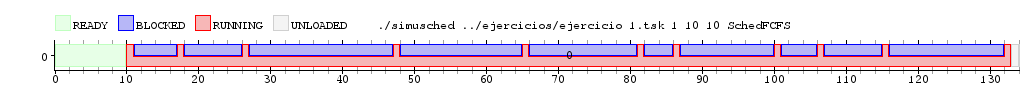
\includegraphics[width=15cm]{../ejercicios/ejercicio 1}
\end{figure}

\section{Ejercicio 2}

El lote de tareas para este ejercicio fue bastante simple, simplemente se compone de dos Tasks que corren desde un principio, el primero un TaskCPU de 100 ciclos, que representa al algoritmo complejo,y el segundo un TaskConsola (implementado en el ejercicio anterior) con 20 llamadas bloqueantes de entre 2 y 4 ciclos cada una, que representaría a la aplicación de musica. Y luego de 80 ciclos se carga otra TaskConsola con 25 llamadas bloqueantes de entre 2 y 4 ciclos cada una, que representa al navegador, para dar cuenta que esta ultima tarea se ejecuto luego de la aplicación de musica.

A continuación veremos como se comportó este lote al cargarse a través de un scheduler con política FCFS, en uno y dos núcleos respectivamente:

\begin{figure}[h!]
\caption{Lote de tareas ejecutándose en 1 núcleo \label{grf:ex2-1}}
\centering
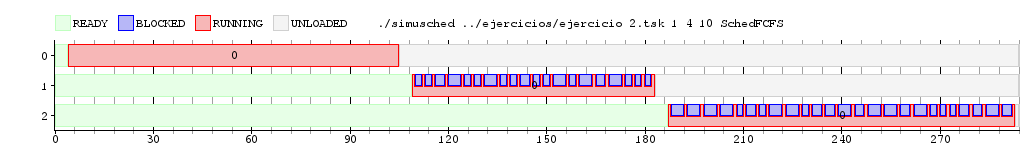
\includegraphics[width=15cm]{../ejercicios/ejercicio 2 - 1 nucleo}
\end{figure}

\begin{figure}[h!]
\caption{Lote de tareas ejecutándose en 2 núcleos \label{grf:ex2-2}}
\centering
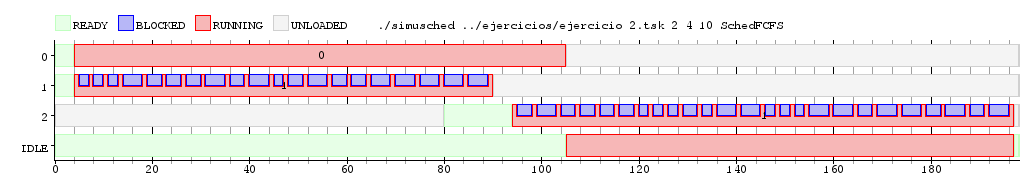
\includegraphics[width=15cm]{../ejercicios/ejercicio 2 - 2 nucleos}
\end{figure}

Como se puede observar, lo que sucede con esta política al aplicarse sobre una maquina de un núcleo, es que se convierte en un planificador secuencial, lo cual es lógico ya que trabaja como una cola, y al haber solo un núcleo, las aplicaciones se van a ir desencolando a medida que se libere ese único núcleo.
Algo muy parecido se puede ver en el caso de planificación con dos núcleos, solo que ahora se puede desencolar para cada núcleo a medida que se liberen, lo que permite una ejecución paralela de tareas.\\
Los tiempos de latencia para la ejecución fueron:
\begin{table}[]
\centering
\caption{Waiting time}
\label{ex2}
\begin{tabular}{ccc}
Task & Cores & Waiting Time \\
0 & 1 & 4 \\
1 & 1 & 109 \\
2 & 1 & 183 \\
0 & 2 & 4 \\
1 & 2 & 4 \\
2 & 2 & 77
\end{tabular}
\end{table}

Una clara conclusión es que, la desventaja de usar esta política en una maquina con un solo núcleo es que, como dijimos previamente, termina ejecutando las aplicaciones en forma secuencial, por lo tanto uno debe esperar a que la primera aplicación deje de correr para que inicie la segunda y así sucesivamente, por lo tanto, y como se ve en el gráfico de forma clara, nunca se podrá trabajar en multitarea, ya que no hay ninguna política para compartir tiempos de procesamiento. En el caso con dos núcleos, no es que hay una política de compartir tiempos sino que, al haber dos núcleos, se pueden utilizar dos aplicaciones al mismo tiempo, pero solo dos, y solo en el orden de la cola principal. Por lo tanto si se quieren realizar varias tareas a la ves lo mejor seria, o tener mas núcleos, o mucho mejor aun, cambiar la política de scheduling por una que implemente tiempos compartidos con, por ejemplo, una implementación por quantums.

\section{Ejercicio 3}

Para esta implementación analizamos las características de las llamadas bloqueantes y llegamos a la conclusión que estas llamadas cuestan el tiempo del bloqueo en si mas 1 ciclo para hacer dicha llamada, por lo tanto en este caso cada bloqueo va a costar realmente 2 ciclos de procesamiento.\par
Por lo tanto la implementación consto en elegir al azar (utilizando un generador de números pseudoaleatorios de la librería estándar de C++) $cantBloqueos$ números aleatorios entre $0$ y $totalCpu - cantBloqueos - 2$.\par
El "$-cantBloqueos$" se contempla para descartar del tiempo total lo que cuesta cada llamada en si, y luego, el "$-2$" sea contempla para que las llamadas no caigan nunca en los últimos dos ciclos de ejecución, ya que esto forzaría a que el tiempo de ejecución total se alargue por culpa del último bloqueo.\par
Estos números, a medida que fueron generados se insertaron en un $set$ para asegurar que no se contemplen dos iguales.\par
Luego de generar todos los números, corremos un ciclo $for$ que va desde $0$ hasta $totalCpu - cantBloqueos - 1$, si el numero de iteración actual se encuentra en el $set$ de números, se realiza un bloqueo de 1 ciclo (el cual consumió entonces 2 ciclos) y, sino se realiza un uso de CPU de 1 ciclo.\par
El lote que realizamos para probar nuestra implementación fue el siguiente:

\begin{verbatim}
TaskBatch 25 3
TaskBatch 90 15
TaskBatch 50 8
\end{verbatim}

Y el resultado gráfico fue:

\begin{figure}[h!]
\caption{Lote de tareas ejecutándose en un núcleo con un costo de cambio de contexto de 4 ciclos \label{grf:ex3}}
\centering
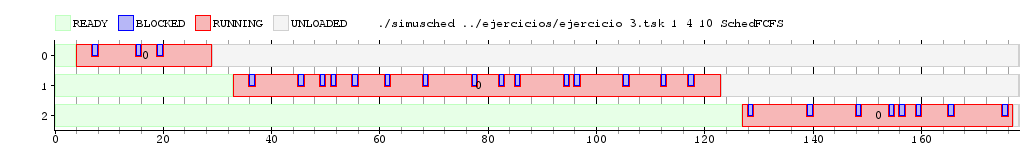
\includegraphics[width=15cm]{../ejercicios/ejercicio 3}
\end{figure}

\section{Ejercicio 5}

Utilizamos el siguiente lote:

\begin{verbatim}
TaskCPU 50
TaskCPU 50
TaskCPU 50
TaskConsola 5 3 3
TaskConsola 5 3 3
\end{verbatim}

Que nos generó las siguientes métricas:

\begin{table}[h!]
\centering
\caption{Métricas para los parámetros pedidos}
\label{tbl:ex5}
\begin{tabular}{ccccc}
Task & Quantum & Latencia & Waiting Time & Tiempo Total \\
0    & 2       & 2        & 288          & 341           \\
1    & 2       & 6        & 291          & 348           \\
2    & 2       & 10       & 294          & 355           \\
3    & 2       & 14       & 84           & 104            \\
4    & 2       & 17       & 87           & 110            \\
0    & 10      & 2        & 162          & 215           \\
1    & 10      & 14       & 165          & 230           \\
2    & 10      & 26       & 168          & 245           \\
3    & 10      & 38       & 201          & 245            \\
4    & 10      & 41       & 204          & 251            \\
0    & 50      & 2        & 114          & 167           \\
1    & 50      & 54       & 117          & 222           \\
2    & 50      & 106      & 120          & 277           \\
3    & 50      & 158      & 177          & 341            \\
4    & 50      & 161      & 180          & 347           
\end{tabular}
\end{table}

Es claro que tomar el quantum 2 minimiza la latencia, ya que vamos a estar realizando context switch muy rápidamente y los procesos no estarán esperando mucho tiempo para ejecutar. Por otro lado, este mismo parámetro maximiza tanto el waiting time como el completion time, lo cual tiene sentido considerando que vamos a estar sufriendo el costo del context switch demasiado seguido.

Por otro lado, tomar un quantum de 10 nos lleva a aumentar ligeramente la latencia y bajar el waiting time, así como a balancear mejor el tiempo total entre todas las tareas. Observemos que en este caso no tenemos tareas que terminen antes de los 251 ticks, pero tampoco tenemos ninguna que termine luego de ese punto, a diferencia de lo que sucede cuando tomamos un quantum de 2.

Finalmente, tomar un quantum de 50 vuelve a aumentar la latencia, bajar aun más el waiting time promedio, pero esta vez tenemos que aumenta el turnaround. Observemos que este quantum tiende a beneficiar a las tareas 0, 1 y 2, por el contrario del quantum 2, que tiende a beneficiar a las tareas 3 y 4.

En conclusión, hemos encontrado que variar el quantum nos lleva a un trade-off entre la latencia, el waiting time, y el tiempo total de ejecución.

\begin{figure}[h!]
\caption{Lote de tareas ejecutado con quantum = 2, cambio de contexto de 2 ciclos, y un sólo núcleo. \label{grf:ex5-1}}
\centering
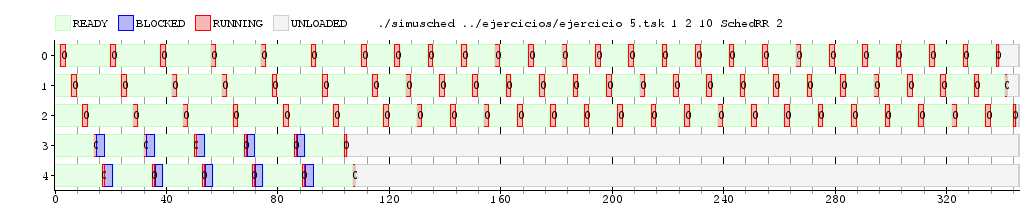
\includegraphics[width=15cm]{../ejercicios/ejercicio 5 - quantum 2}
\end{figure}

\begin{figure}[h!]
\caption{Lote de tareas ejecutado con quantum = 10, cambio de contexto de 2 ciclos, y un sólo núcleo. \label{grf:ex5-10}}
\centering
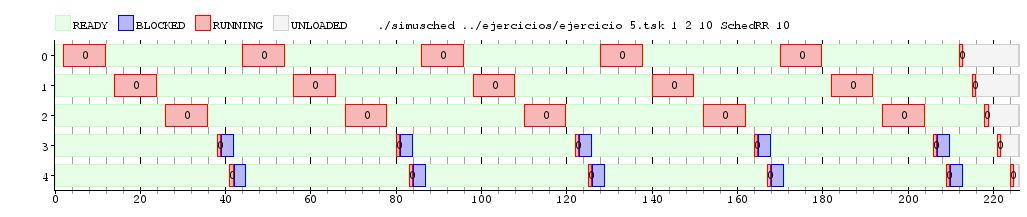
\includegraphics[width=15cm]{../ejercicios/ejercicio 5 - quantum 10}
\end{figure}

\begin{figure}[h!]
\caption{Lote de tareas ejecutado con quantum = 50, cambio de contexto de 2 ciclos, y un sólo núcleo. \label{grf:ex5-50}}
\centering
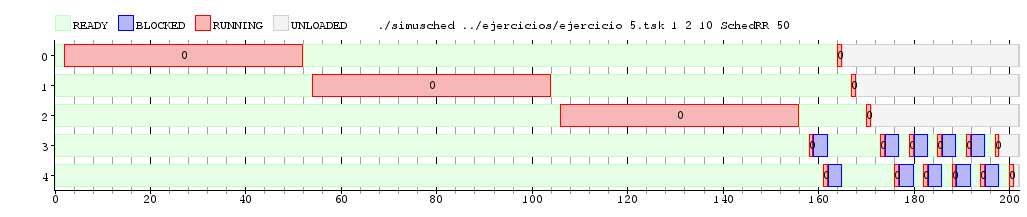
\includegraphics[width=15cm]{../ejercicios/ejercicio 5 - quantum 50}
\end{figure}

\section{Ejercicio 6}

\begin{table}[h!]
\centering
\caption{Métricas para el scheduler con FCFS}
\label{tbl:ex6}
\begin{tabular}{cccc}
Task & Latencia & Waiting Time & Tiempo Total \\
0    & 2        & 2            & 55           \\
1    & 55       & 55           & 161           \\
2    & 108      & 108          & 267           \\
3    & 161      & 161          & 343           \\
4    & 184      & 184          & 389          
\end{tabular}
\end{table}

Queda claro, observando las métricas, que en términos de tiempo total ambos algoritmos son similares: el tiempo total promedio utilizando FCFS es de 243, mientras que utilizando Round Robin son de 251.6, 237.2, y 270.8 (para los quantums 2, 10 y 50 respectivamente).

La diferencia está absolutamente en cómo deseamos distribuir la prioridad: FCFS claramente prioriza a los procesos que vinieron primero, mientras que Round Robin realiza una distribución más equitativa del tiempo. Entre otras cosas, el hecho de usar Round Robin permite aprovechar el tiempo en el cual una tarea se encuentra bloqueada para asignarle ese tiempo a otra tarea, así como de crear la ilusión de que más de una tarea se corre al mismo tiempo. Ambas cuestiones no suceden en un esquema de scheduling que utilice FCFS.

Tal vez la desventaja más grande de FCFS sea precisamente esta última: no es apto para un entorno multiusuario, ya que un solo usuario podría crear muchos procesos y dejar a otro usuario sin recursos por un largo período de tiempo, mientras que el esquema de Round Robin no permitite estas situaciones.

\begin{figure}[h!]
\caption{Lote de tareas ejecutado sobre FCFS con cambio de contexto de 2 ciclos, y un sólo núcleo. \label{grf:ex6-1}}
\centering
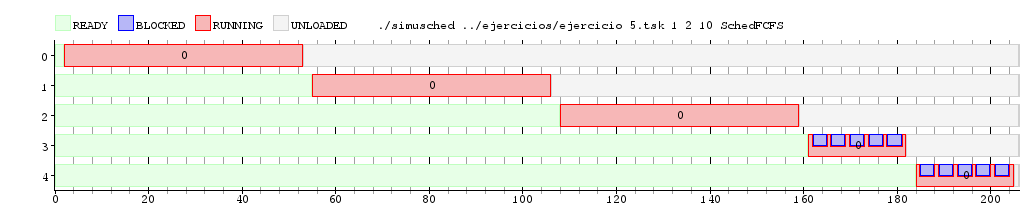
\includegraphics[width=15cm]{../ejercicios/ejercicio 6 - quantum 2}
\end{figure}

\section{Ejercicio 7}

Comenzamos con el lote

\begin{verbatim}
TaskCPU 200
@20:
TaskCPU 200
\end{verbatim}

\begin{figure}[h!]
\caption{Primer lote de tareas \label{grf:ex7-1}}
\centering
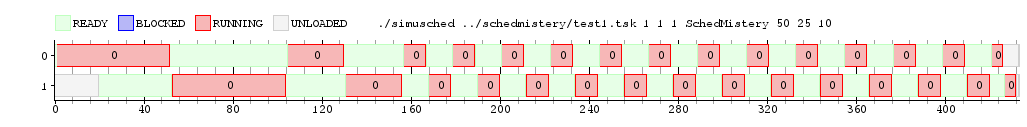
\includegraphics[width=15cm]{../ejercicios/ejercicio 7-1}
\end{figure}

Utilizando todos los argumentos del programa en 1, y pasando como único argumento del scheduler al 1 también. Luego probamos con pasar 5, 10, y después comenzamos a agregar argumentos. Esto nos permitió darnos cuenta que el quantum de tiempo para las tareas debía corresponderse con los argumentos. Y que, mas fuertemente, que estos quantums son asignados en orden para cada tarea y, al llegar al ultimo, este es el unico que se sigue asignadno. Luego, utilizamos el siguiente lote de tareas:

\begin{verbatim}
*3 TaskAlterno 0 1 0 1 0 1 1
TaskCPU 10
@4:
TaskCPU 10
@30:
*3 TaskAlterno 0 1 0 1 0 1 1
TaskCPU 10
\end{verbatim}

\begin{figure}[h!]
\caption{Resultado del segundo lote de tareas \label{grf:ex7-2}}
\centering
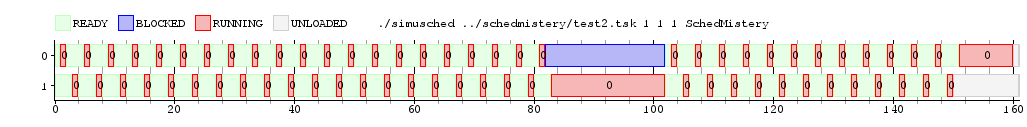
\includegraphics[width=15cm]{../ejercicios/ejercicio 7-2}
\end{figure}

Que nos mostró que el scheduler de la cátedra baja el quantum de los procesos al valor anterior cuando se bloquean, así como que el primer quantum debe ser uno. Finalmente, testeamos que este andando bien corriendo varios ejemplos, que se pueden encontrar en la carpeta \verb`schedmistery`.

\section{Ejercicio 8}

\end{document}